% !TeX root = ../libro.tex
% !TeX encoding = utf8


\chapter{Introducción}

\noindent Actualmente, las \textbf{Redes Neuronales Convolucionales} (CNN\footnote{Convolutional Neural Network}) son una de las herramientas más usadas de la Inteligencia Artificial. De hecho, son el principal objeto de estudio del \textbf{Deep Learning}, una rama del \textit{Aprendizaje Automático} (AA) en la que hoy en día se está invirtiendo mucho esfuerzo en invesitgar y de la que, anualmente, se publican muchos artículos. Destaca, especialmente, el excelente desempeño que tienen en el procesamiento de imágenes para tareas de clasificación, segmentación o incluso generación de nuevas imágenes. Es por ello que, en el presente trabajo, nos proponemos intentar realizar una \textbf{modelización matemática} de este tipo de redes, para conocerlas mejor desde un punto de vista más teórico y poder demostrar una de sus principales propiedades: \textbf{la invarianza por traslaciones}.

\medskip

\noindent Uno de los principales problemas en el ámbito del AA y la visión por computador es el de clasificación de imágenes y detección de objetos en las mismas. En este contexto, definimos el concepto de \textbf{invarianza} como la capacidad de reconocer un objeto en una imagen incluso si su apariencia ha variado en algún sentido (mediante una rotación, una  ligera deformación o una traslación). Esto es algo muy importante, pues nos indica que se preserva la identidad del objeto incluso a pesar de haberse sometido a ciertos cambios.

\medskip

\noindent De esta forma definimos la \textbf{invarianza por traslaciones} \cite{DBLP:journals/corr/abs-1801-01450} como la capacidad de reconocer la identidad de un objeto en una imagen incluso si este se ha desplazado (véase la \autoref{fig:invarianza_traslaciones}). Esta propiedad es fundamental y sabemos que las CNN la verifican.

\begin{figure} [!h]
    \centering
    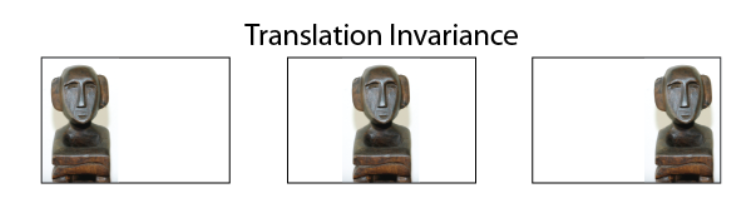
\includegraphics[width=0.8\textwidth]{img/translation_invariance.png}
    \caption{Los tres coches deben identificarse como iguales, aunque se ecuentren desplazados.}
    \label{fig:invarianza_traslaciones}
\end{figure}

\medskip

\noindent Otra propiedad importante es la \textbf{invarianza frente a pequeñas deformaciones} (difeomorfismos, véase la \autoref{fig:difeomorfismo}), que es la capacidad de reconocer la identidad de un objeto en una imagen a pesar de que este pueda haber sido alterado con pequeñas deformaciones (véase la \autoref{fig:deformaciones_5} y \autoref{fig:deformaciones_1}).


\begin{figure}[!h]
  \centering
  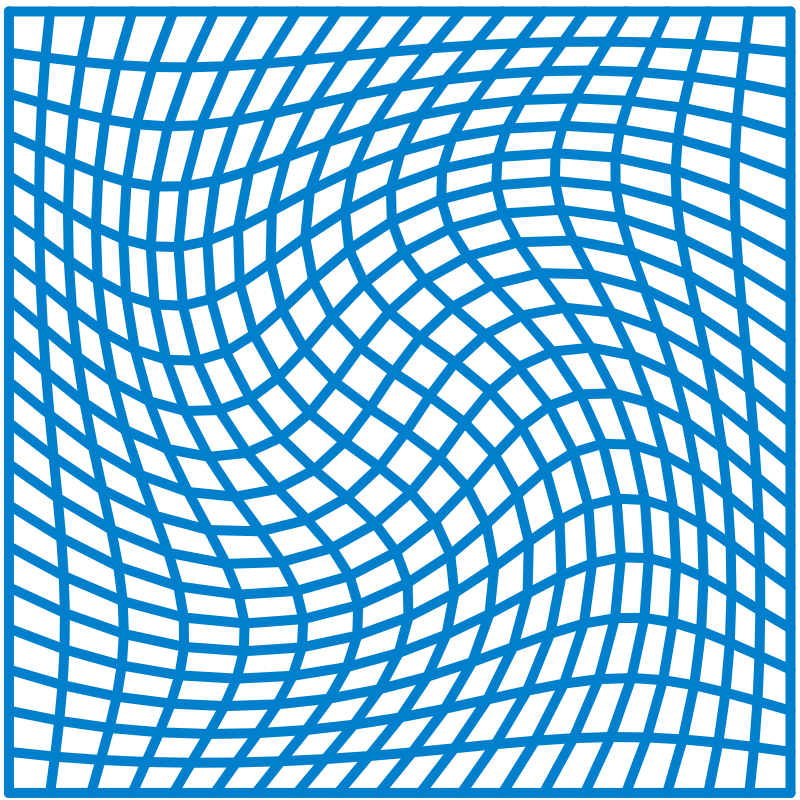
\includegraphics[width=0.5\textwidth]{img/Diffeomorphism.png}
  \caption{Acción de un difeomorfismo en una rejilla.}
  \label{fig:difeomorfismo}
\end{figure}

\begin{figure}[!h]
  \centering
  
\includegraphics[width=0.8\textwidth]{img/5_deformado.png}
  \caption{Todas las imágenes deberían clasificarse como 5, pese a las deformaciones.}
  \label{fig:deformaciones_5}
\end{figure}

\begin{figure}[!h]
  \centering
  
\includegraphics[width=0.5\textwidth]{img/1_excesivamente_deformado.png}
  \caption{Deformación excesiva que permite confundir el 1 con el 2 cuando se le aplica el difeomorfismo. Por eso nos centramos en \entrecomillado{pequeñas} deformaciones, para no alterar la identidad del objeto en la imagen.}
  \label{fig:deformaciones_1}
\end{figure}

\medskip


\noindent Realizaremos nuestro estudio sobre las funciones $L^2(\mathbb{R}^d)$. En este espacio buscaremos un operador que sea Lipschitz-continuo por la acción de difeomorfismos y que mantenga información de alta frecuencia para diferenciar entre distintos tipos de señales.

\medskip

\noindent La invarianza por traslaciones, entendida en el contexto de las imágenes puede verse como trasladar cada pixel de la imagen en una misma dirección la misma distancia. En este sentido definimos las traslaciones de funciones de cuadrado integrable: 

\begin{definicion}
$L_cf(x)=f(x-c)$ es la traslación de $f \in L^2(\mathbb{R}^d)$ por $c \in \mathbb{R}^d$ .
\end{definicion}

\medskip

\noindent Así, decimos que un operador $\Phi$ sobre  $L^2(\mathbb{R}^d)$, es invariante por traslaciones si $\Phi(L_cf(x))=\Phi(f)$ para todo $f \in L^2(\mathbb{R}^d)$ y para todo $c \in \mathbb{R}^d$. En el siguiente apartado trataremos el caso del módulo de la transformada de Fourier de $f$ como un ejemplo de un operador invariante por traslaciones, aunque la aparición de inestabilidades frente a deformaciones en las altas frecuencias nos obligará a descartarlo como opción para la modelización de CNN, pues no preserva la Lipschitz-continuidad frente a difeomorfismos.

\medskip

\noindent Para preservar la estabilidad en $L^2(\mathbb{R}^d)$ queremos que $\Phi$ sea no-expansiva.

\begin{definicion}
Decimos que $\Phi$ es no-expansiva si: 
$$\forall f,h \in L^2(\mathbb{R}^d)\; \| \Phi(f)-\Phi(h)\| \leq \|f-h\|$$
\end{definicion}

\noindent donde $\| f\|$ denota la norma de $f$ en  $L^2(\mathbb{R}^d)$.


\begin{definicion}
  Una función diferenciable $f: \mathbb{R}^d \rightarrow \mathbb{R}^d$, es un \textit{difeomorfismo} si $f$ es una biyección y su inversa $f^{-1}:\mathbb{R}^d \rightarrow X$ es también diferenciable. 
\end{definicion}


\noindent En nuestro caso, vamos a encargarnos de verificar la Lipschitz-continuidad relativa a la acción de pequeños difeomorfismos cercanos a las traslaciones. Dichos difeomorfismos transforman $x \in \mathbb{R}^d$ en $x-\tau (x)$ donde $\tau$ es el campo de desplazamiento. 

\begin{definicion}
Denotemos $L_{\tau} f(x)=f(x-\tau(x))$ como la acción del difeomorfismo $\mathbb{1}-\tau$ sobre $f$.
\end{definicion} 

\medskip

\noindent Recordemos que la condición de Lipschitz es la siguiente: 

\begin{definicion}
  Sea $f: M \rightarrow N$ una función entre dos espacios métricos $M$ y $N$ con sus respectivas distancias $d_M$ y $d_N$. Se dice que $f$ satisface la condición de Lipschitz si $\exists C>0$ tal que: 

  $$d_N(f(x),f(y))\leq C d_M(x,y), \; \; \forall x,y \in M$$
\end{definicion}

\noindent En nuestro caso, dado que el espacio de partida es $L^2(\mathbb{R}^d)$ y los puntos que vamos a comparar son las funciones $f$ y $L_\tau f=f(x-\tau(x))$ sabemos que $\|\Phi(f) - \Phi(L_cf) \|$ estará acotada por $\|f\| · d(\mathbb{1}, \mathbb{1}-\tau)$, de manera que necesitamos definir una distancia entre el difeomorfismo $\mathbb{1}$ y $\mathbb{1}-\tau$. 

\begin{definicion}
Se define una distancia entre $\mathbb{1}-\tau$ y $\mathbb{1}$ en cualquier subconjunto compacto $\Omega$ de $\mathbb{R}^d$ como 

\begin{equation} \label{eq::distancia}
  d_\Omega(\mathbb{1},\mathbb{1}-\tau) = \sup_{x \in \Omega} |\tau (x)| + \sup_{x \in \Omega} |\nabla \tau (x)| + \sup_{x \in \Omega}|H \tau (x)|
\end{equation}

\end{definicion}
\medskip

\noindent Donde $|\tau (x)|$ es la norma euclídea en $\mathbb{R}^d$, $|\nabla \tau (x)|$ es la norma del supremo de la matriz jacobiana $\nabla \tau (x)$, y $|H \tau (x)|$ es la norma del supremo del Hessiano.

\medskip

\noindent No obstante, debido a que trataremos con funciones que son invariantes por traslaciones, la condición de Lipschitz será independiente de la amplitud máxima de la traslación $\sup_{x \in \mathbb{R}^d}|\tau (x)|$, es por ello que obviaremos este término. 

\medskip


\noindent En lo que sigue vamos a denotar: 

\begin{itemize}
  \item $||\nabla \tau ||_\infty := \sup_{x \in \mathbb{R}^d} |\nabla \tau(x)|$
  \item $||H \tau ||_\infty := \sup_{x \in \mathbb{R}^d} |H \tau(x)|$ 
\end{itemize}

\medskip

\noindent Así, podemos finalmente expresar la condición de Lipschitz que un operador debería satisfacer en nuestro caso como: 


\medskip

\begin{definicion} \label{def::Lipschitz_cont}
\noindent Un operador invariante por traslaciones $\Phi$ se dice \entrecomillado{Lipchitz-continuo} por la acción de los difeomorfismos $C^2$  si para cualquier compacto $\Omega \subset \mathbb{R}^d$ existe una constante $C$ tal que para todo $f \in L^2(\mathbb{R}^d)$ con soporte en $\Omega$ y para todo $\tau \in C^2(\mathbb{R}^d)$ se cumple:

\begin{equation} \label{eq::Lipschitz_condition}
  \| \Phi(f)-\Phi(L_{\tau}f)\|_\mathcal{H} \leq C\|f\|(\|\nabla\tau\|_{\infty} + \|H \tau\|_\infty).
\end{equation}
\end{definicion}

\medskip

\noindent La continuidad Lipschitz de \eqref{eq::Lipschitz_condition} implica que $\Phi$ es invariante por traslaciones globales, pero dicha condición es mucho más fuerte: \eqref{eq::Lipschitz_condition} garantiza que $\Phi$ se ve poco afectada por los términos de primer y segundo grado de difeomorfismos que son traslaciones locales.

\medskip


\noindent Una vez presentadas las principales herramientas con las que trabajaremos, veremos en las futuras secciones cómo, para solucionar el problema, se optará por utilizar \textbf{transformadas de ondeletas}. Aunque esto abre nuevos frentes como el hecho de que estas \textbf{no son invariantes por traslaciones}. Para lograr la invarianza por traslaciones será necesario componer la transformada con un \textbf{operador no lineal} para obtener coeficientes invariantes. Este nuevo operador consistirá en una \textbf{cascada de convoluciones} de operadores no lineales y no conmutativos de manera que cada uno de ellos calcula el módulo de la transfomada de odeletas, y será este nuevo operador el que podremos interpretar como la modelización matemática de una CNN.


\endinput